\section{Chapter 1: Nuclear Energy and Fusion}

\subsection{Give a historical perspective of the controlled use of nuclear energy in general and fusion in particular.}
\solutionblock{In the early days scientists dreamed about changing Lead into Gold. With better knowledge of chemical reactions they at least tried but were doomed to fail from the beginning.\\ At the end of the 19th century scientists discovered that atoms are not the smallest particles and that they can be split. Especially the discovery of radiation and radioactive decay was a big step forward.\\ Looking at the sun, they wondered how it could burn for so long. The answer was nuclear fusion and Einstein gave us the world famous formula $E = m c^2$ in 1905, which relates energy and mass. Yet it was Francis Aston's discovery or rather precise measurement of the mass of Helium and Hydrogen that gave us the final piece of the puzzle. He measured that the mass of Helium was less than the mass of 4 Hydrogen atoms and postulated that the difference in mass was converted to energy by a nuclear reaction.\\ Only in the late 20s a complete understanding of the nuclear fusion process was achieved by also taking quantum mechanics into account (otherwise the sun would have been to cold for any reaction to take place).\\
In the late 30s Otto Hahn and Fritz Strassmann discovered nuclear fission of uranium by bombarding it with neutrons.

\textbf{Fission:} After the second world war first attempts were made to build a fusion reactor. The idea was to fuse deuterium and tritium together to form Helium. Deuterium is a Hydrogen Isotope naturally found in water and tritium was made using Lithium in so called breeder reactors. The US, UK and Soviet Union all started their classified fusion programs in the 50s. First the confinement was done using magnetic fields, this turned out to be very difficult. Later the idea of inertial confinement was born with the invention of the laser (1960). There a laser is used to insert energy into a pellet of fuel which then is only confined by its own inertia.\\
Both inertial and magnetic confinement fusion are still being researched today and are the most promising ways to achieve fusion in a viable way.\\}

\subsection{Draw and explain a schematic fusion power plant.}
\solutionblock{
\textbf{A note on Li:} To get tritium for the fusion reaction Lithium is used as a blanket around the plasma. The neutrons from the fusion reaction hit the Lithium and produce tritium.\\\\
Like a nuclear fission plant a fusion plant is also a thermal power plant using the heat from the fusion reaction to produce steam and drive a turbine.\\
\begin{figure}[H]
    \centering
    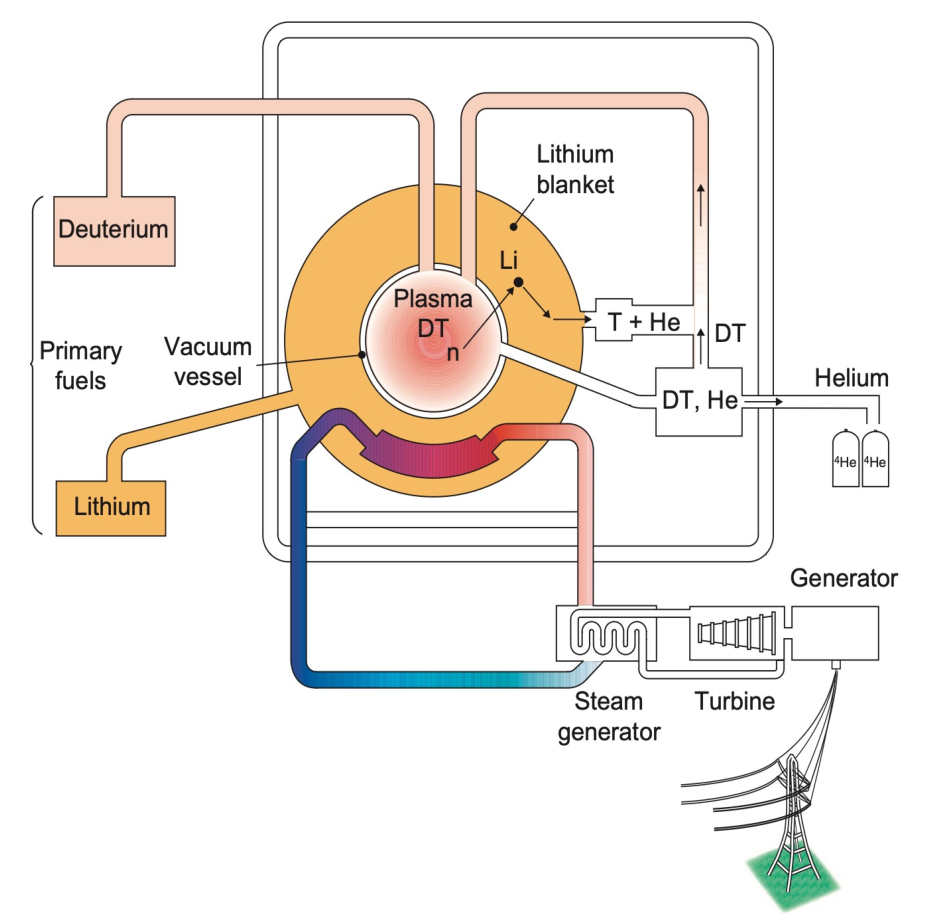
\includegraphics[width=0.8\textwidth]{chapters/fig/1_fusion_power_plant.png}
    \caption{Schematic diagram of nuclear fusion power plant}
    \label{fig:fusion_power_plant}
\end{figure}
}

\subsection{Explain the difference between magnetic and inertial confinement fusion.}
\solutionblock{Magnetic confinement fusion uses magnetic fields (e.g. tokamak) to confine the plasma and inertial confinement fusion uses lasers to heat up a pellet of fuel and then uses the inertia of the pellet to confine the plasma.\\}
